%%%%%%%%%%%%%%%%%%%%%%%%%%%%%%%%%%%%%%%%%
% Document Author: Plinio H. Vargas
% Course: CS-532, Spring 2016 at Old Dominion University
%
% Structured General Purpose Assignment
% LaTeX Template
%
% This template has been downloaded from:
% http://www.latextemplates.com
%
% Original template author:
% Ted Pavlic (http://www.tedpavlic.com)
%
% Note:
% The \lipsum[#] commands throughout this template generate dummy text
% to fill the template out. These commands should all be removed when 
% writing assignment content.
%
%%%%%%%%%%%%%%%%%%%%%%%%%%%%%%%%%%%%%%%%%
%----------------------------------------------------------------------------------------
%	PACKAGES AND OTHER DOCUMENT CONFIGURATIONS
%----------------------------------------------------------------------------------------

\documentclass{article}

\usepackage{fancyhdr} % Required for custom headers
\usepackage{lastpage} % Required to determine the last page for the footer
\usepackage{extramarks} % Required for headers and footers
\usepackage{listings}
\usepackage{graphicx} % Required to insert images
\usepackage{lipsum} % Used for inserting dummy 'Lorem ipsum' text into the template
\usepackage[bookmarks,bookmarksopen,bookmarksdepth=2]{hyperref} % for bookmarks
\usepackage{enumerate}
\usepackage{csquotes} % for quoting things
\usepackage{multirow}
\usepackage{amsmath}
\usepackage{caption}
\usepackage{navigator}%\usepackage{caption}
\usepackage[shortlabels]{enumitem}
\usepackage{enumitem}
\usepackage{lmodern}
\usepackage[utf8]{inputenc}
%\usepackage[table]{xcolor}% http://ctan.org/pkg/xcolo
\usepackage[dvipsnames]{xcolor}
\usepackage{longtable}
\usepackage{textcomp}
\usepackage{url}
\usepackage{import}
\usepackage{float}
\usepackage{dashrule} % for dashline
\usepackage{keystroke}
\usepackage{amssymb}
\usepackage{booktabs}

\lstdefinestyle{numbers}
{ frame=tb,
  language=python,
  aboveskip=3mm,
  belowskip=3mm,
  showstringspaces=false,
  columns=flexible,
  basicstyle={\small\ttfamily},
  numbers=left,
  numberstyle=\tiny\color{gray},
  keywordstyle=\color{blue},
  commentstyle=\color{OliveGreen},
  stringstyle=\color{purple},
  breaklines=true,
  breakatwhitespace=true,
  tabsize=3
}

\lstdefinestyle{nonumbers}
{ frame=shadowbox,
  language=python,
  aboveskip=3mm,
  belowskip=3mm,
  showstringspaces=false,
  columns=flexible,
  basicstyle={\small\ttfamily},
  numbers=none,
  numberstyle=\tiny\color{gray},
  keywordstyle=\color{blue},
  commentstyle=\color{OliveGreen},
  stringstyle=\color{purple},
  breaklines=true,
  breakatwhitespace=true,
  tabsize=3
}

\lstdefinestyle{mybox}
{
	basicstyle={\small\ttfamily},
    numbers=left,
    numberstyle=\tiny\color{gray},
    stepnumber=1,
    numbersep=5pt,
    showspaces=false, % don't show spaces by adding underscores
    showstringspaces=false, % don't underline spaces in strings
    showtabs=false, % don't show tabs with underscores
    frame=shadowbox,
    tabsize=4,
    captionpos=b,
    breaklines=true,
    breakatwhitespace=false,
  	keywordstyle=\color{blue},
	commentstyle=\color{OliveGreen},
  	stringstyle=\color{purple},    
    rulesepcolor=\color{red!20!green!20!blue!20},
    numberbychapter=false,
    stringstyle=\color{purple},
}


\providecommand{\providehyphenmins}[2]{}

% Margins
\topmargin=-0.45in
\evensidemargin=0in
\oddsidemargin=0in
\textwidth=6.5in
\textheight=9.0in
\headsep=0.25in 

\linespread{1.1} % Line spacing
\newcommand*{\medtau}{\mathbin{\scalebox{1.5}{$\tau$}}}% increase size of tau
\newcommand*{\medtaub}{\mathbin{\scalebox{1.5}{$\tau_b$}}}% increase size of tau_b
\newcommand\multibrace[3]{\rdelim\}{#1}{3mm}[\pbox{#2}{#3}]}

% Set up the header and footer
\pagestyle{fancy}
\lhead{\hmwkAuthorName} % Top left header
\chead{\hmwkShortClass\ (\hmwkClassInstructor\ \hmwkClassTime): \hmwkShortTitle} % Top center header
%\rhead{\firstxmark} % Top right header
\rhead{} % Top right header
\lfoot{\lastxmark} % Bottom left footer
\cfoot{} % Bottom center footer
\rfoot{Page\ \thepage\ of\ \pageref{LastPage}} % Bottom right footer
\renewcommand\headrulewidth{0.4pt} % Size of the header rule
\renewcommand\footrulewidth{0.4pt} % Size of the footer rule

\setlength\parindent{0pt} % Removes all indentation from paragraphs

%----------------------------------------------------------------------------------------
%	DOCUMENT STRUCTURE COMMANDS
%	Skip this unless you know what you're doing
%----------------------------------------------------------------------------------------

% Header and footer for when a page split occurs within a problem environment
\newcommand{\enterProblemHeader}[1]{
\nobreak\extramarks{#1}{#1 continued on next page\ldots}\nobreak
\nobreak\extramarks{#1 (continued)}{#1 continued on next page\ldots}\nobreak
}

% Header and footer for when a page split occurs between problem environments
\newcommand{\exitProblemHeader}[1]{
\nobreak\extramarks{#1 (continued)}{#1 continued on next page\ldots}\nobreak
\nobreak\extramarks{#1}{}\nobreak
}

\newcounter{sub}[section]
\newenvironment{sub}[1][]{\stepcounter{sub}\thesub #1}{ }

\setcounter{secnumdepth}{3} % Removes default section numbers
\newcounter{homeworkProblemCounter} % Creates a counter to keep track of the number of problems
\newcommand{\sectionNumber}{\arabic{homeworkProblemCounter}.\sub }


\newcommand{\homeworkProblemName}{}
\newenvironment{homeworkProblem}[1][Problem \arabic{homeworkProblemCounter}]{ % Makes a new environment called homeworkProblem which takes 1 argument (custom name) but the default is "Problem #"
\stepcounter{homeworkProblemCounter} % Increase counter for number of problems
\setcounter{sub}{0}
\renewcommand{\homeworkProblemName}{#1} % Assign \homeworkProblemName the name of the problem
\
\section{\homeworkProblemName} % Make a section in the document with the custom problem count
\enterProblemHeader{\homeworkProblemName} % Header and footer within the environment
}{
\exitProblemHeader{\homeworkProblemName} % Header and footer after the environment
}

\newcommand{\problemAnswer}[1]{ % Defines the problem answer command with the content as the only argument
\noindent\framebox[\columnwidth][c]{\begin{minipage}{0.98\columnwidth}#1\end{minipage}} % Makes the box around the problem answer and puts the content inside
}

\newcommand{\homeworkSectionName}{}
\newenvironment{homeworkSection}[1]{ % New environment for sections within homework problems, takes 1 argument - the name of the section
\renewcommand{\homeworkSectionName}{#1} % Assign \homeworkSectionName to the name of the section from the environment argument
\subsection{\homeworkSectionName} % Make a subsection with the custom name of the subsection
\enterProblemHeader{\homeworkProblemName\ [\homeworkSectionName]} % Header and footer within the environment
}{
\enterProblemHeader{\homeworkProblemName} % Header and footer after the environment
}
   
%----------------------------------------------------------------------------------------
%	NAME AND CLASS SECTION
%----------------------------------------------------------------------------------------

\newcommand{\hmwkTitle}{\\Assignment\ \#1: \\Ex 1.1, 3.7, 3.8, 3.9, 3.14} % Assignment title
\newcommand{\hmwkShortTitle}{Assignment 1} % Assignment title
\newcommand{\hmwkDueDate}{Thursday,\ September 22,\ 2016} % Due date
\newcommand{\hmwkClass}{CS-734/834 Introduction to Information Retrieval} % Course/class
\newcommand{\hmwkShortClass}{CS-734/834 Intro to IR} % Course/class
\newcommand{\hmwkClassTime}{- Fall 2016} % Class/lecture time
\newcommand{\hmwkClassInstructor}{Dr.  Michael L. Nelson} % Teacher/lecturer
\newcommand{\hmwkAuthorName}{Plinio Vargas} % Your name
\newcommand{\hmwkAuthorEmail}{pvargas@cs.odu.edu} % Your name
%------------------------------------------------------------
% Algorithm declaration
%------------------------------------------------------------
\lstnewenvironment{algorithm}[1][] %defines the algorithm listing environment
{   
    %\refstepcounter{nalg} %increments algorithm number
    \captionsetup{labelsep=colon} %defines the caption setup for: it ises label format as the declared caption label above and makes label and caption text to be separated by a ':'
    \lstset{ %this is the stype
        frame=tB,
        numbers=left, 
        mathescape=true,
        numberstyle=\tiny,
        basicstyle={\small\ttfamily}, 
        keywordstyle=\color{blue}\bfseries\em,
        keywords={,input, output, return, 
                   datatype, function, in, 
                   if, else, for, foreach, 
                   while, write, begin, end, 
        } %add the keywords you want, or load a language as Rubens explains in his comment above.
        numbers=left,
        xleftmargin=.04\textwidth,
        #1 % this is to add specific settings to an usage of this environment (for instnce, the caption and referable label)
    }
}
{}
%----------------------------------------------------------------------------------------
%	TITLE PAGE
%----------------------------------------------------------------------------------------

\title{
\vspace{2in}
\textmd{\textbf{\hmwkClass:\ \hmwkTitle}}\\
\normalsize\vspace{0.1in}\small{Due\ on\ \hmwkDueDate}\\
\vspace{0.1in}\large{\textit{\hmwkClassInstructor\ }}
\vspace{3in}
}

\author{\textbf{\hmwkAuthorName} \\ \hmwkAuthorEmail}
\date{} % Insert date here if you want it to appear below your name

%----------------------------------------------------------------------------------------
%	EMBEDDED FILE
%----------------------------------------------------------------------------------------
%\embeddedfile{KarateClub}{../KarateClub.py}
%\embeddedfile{DrawOriginalClub}{../DrawOriginalClub.py}
%----------------------------------------------------------------------------------------
%	START OF DOCUMENT
%----------------------------------------------------------------------------------------
\begin{document}

\clearpage\maketitle
\thispagestyle{empty}

%----------------------------------------------------------------------------------------
%	TABLE OF CONTENTS
%----------------------------------------------------------------------------------------

%\setcounter{tocdepth}{1} % Uncomment this line if you don't want subsections listed in the ToC

\newpage
\clearpage\tableofcontents
\listoffigures
\lstlistoflistings
%\listoftables

\thispagestyle{empty}
\newpage
\setcounter{page}{1}

%Exercices on pages: 35,52,
%----------------------------------------------------------------------------------------
%	Problem 1
%----------------------------------------------------------------------------------------
\begin{homeworkProblem}[Exercise 1.1]% Custom section title
\vspace*{10pt} % Question
Think up and write down a small number of queries for a web search engine.
Make sure that the queries vary in length (i.e., they are not all one word). Try
to specify exactly what information you are looking for in some of the queries.
Run these queries on two commercial web search engines and compare the top
10 results for each query by doing relevance judgments. Write a report that answers
at least the following questions: What is the precision of the results? What
is the overlap between the results for the two search engines? Is one search engine
clearly better than the other? If so, by how much? How do short queries perform
compared to long queries?\\

\subsection{Approach}
I was interested in finding out the recipe of a Latin-American dish called \textbf{Maduro}. \textbf{Google} and \textbf{Bing} were the two search engines used to compare the relevance of the top 10 webpages returned. The experiment started by typing two keywords: \textbf{Maduro plate}.\\

For our purpose, we will use the top 10 results as the total number of retrieved documents.
To compare the precision between the two searches, we can use the formula:
\begin{equation}
   precision = \frac{\left|\{relevant\ documents\} \cap \{retrieved\ documents\}\right|}{\left|\{retrieved\ documents\}\right|}
\end{equation}

\subsubsection{2-Word Query}
%--------------
%  P1 2W Query Google
%--------------
Google Results:\\
The top four queries returned were related to a cigar brand and Venezuelan President: Nicolas Maduro. There were three sites ranked 5\textsuperscript{th}, 6\textsuperscript{th} and 8\textsuperscript{th}, related to Maduro as a dish, but did not included the recipe. See Figure \ref{fig:google1}\\

\begin{figure}\caption{Google Keyword Search \textbf{Maudro Plate}} \label{fig:google1}
	\center
	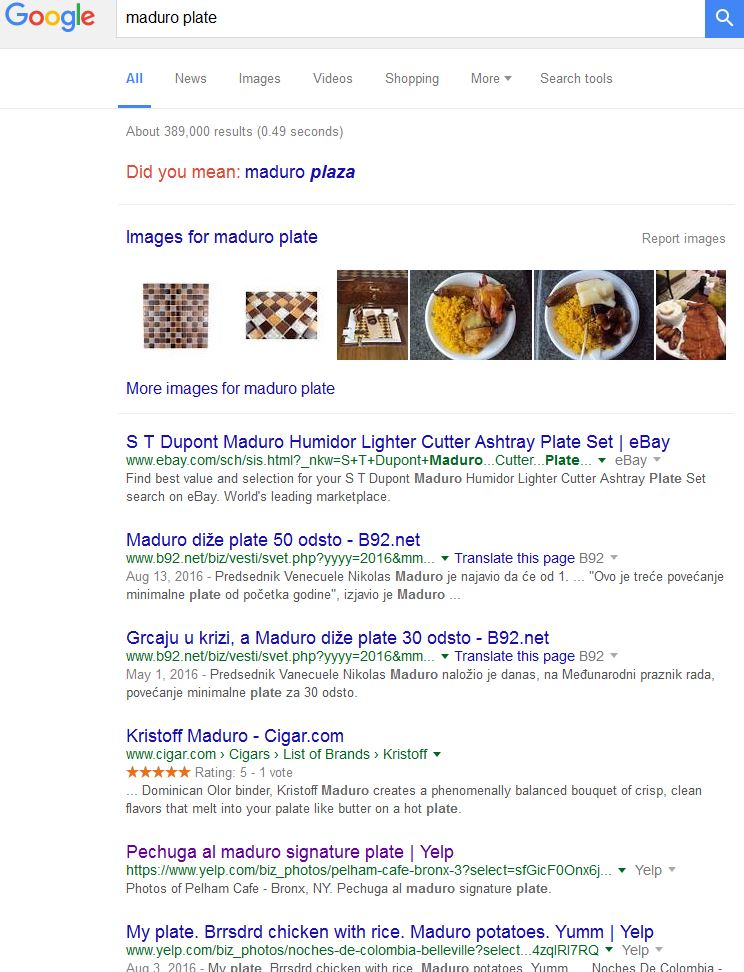
\includegraphics[scale=0.5]{images/Google1.JPG}
\end{figure} 
%--------------
%  P1 2W Query Bing
%--------------
Bing Results:\\
The 1\textsuperscript{st} and 7\textsuperscript{th} were in fact Maduro dish recipes. The 3\textsuperscript{rd}, 6\textsuperscript{th} and 9\textsuperscript{th} were related to a Maduro dish, but they did not provide a recipe. The remaining sites were related to the Maduro cigar brand. See Figure \ref{fig:bing1}\\

\begin{figure}\caption{Bing Keyword Search \textbf{Maudro Plate}} \label{fig:bing1}
	\center
	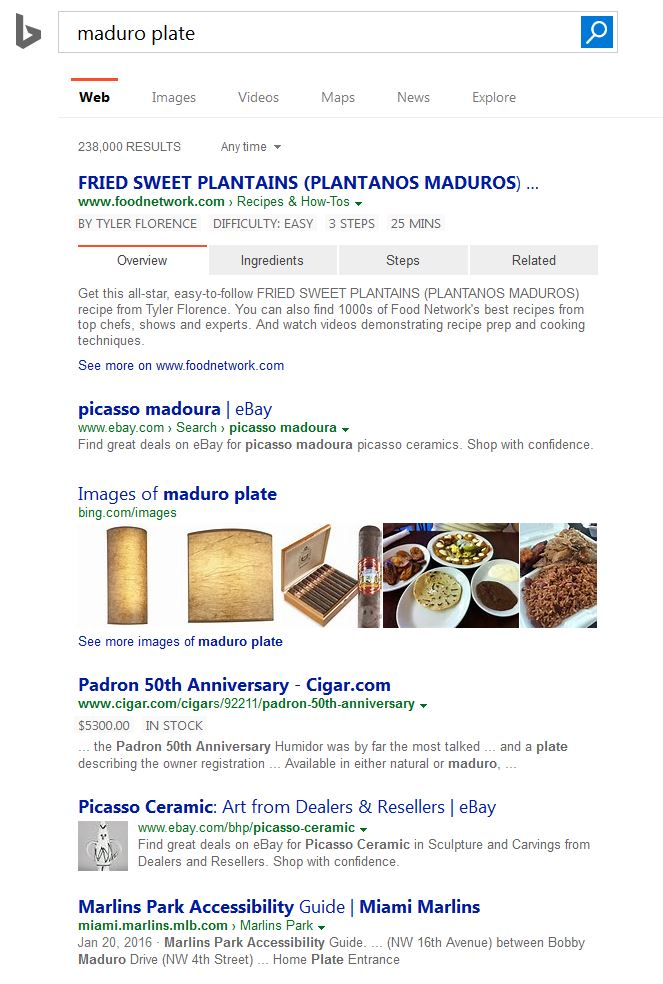
\includegraphics[scale=0.5]{images/Bing1.JPG}
\end{figure} 

%
First query precision calculation for keyword: \textbf{Maduro plate}\\

\begin{equation*}
   Google\ precision = \frac{\left|\{\ \} \cap \{1\cdots 10\}\right|}{\left|10\right|} = 0
\end{equation*}
\begin{equation*}
   Bing\ precision = \frac{\left|\{1,7\} \cap \{1\cdots 10\}\right|}{\left|10\right|} = \frac{1}{5}
\end{equation*}
%
\vspace{3mm}\\
\subsubsection{3-Word Query}
For the second query, three keywords were typed: \textbf{Maduro plantain plate}\\
%--------------
%  P1 3W Query Google
%--------------
Google Results:\\
The top result returned was a Wiki page containing plantain information. The remaining 9 results included Maduro recipe information.\\

%--------------
%  P1 3W Query Bing
%--------------
Bing Results:\\
The 1\textsuperscript{st}, 2\textsuperscript{nd}, 4\textsuperscript{th}, 5\textsuperscript{th}, 6\textsuperscript{th}, 7\textsuperscript{th}, 8\textsuperscript{th} and 10\textsuperscript{th} were in fact Maduro dish recipes. The remaining sites were related to Maduros, but did not contain a recipe.\\

Precision calculation for the 3 keyword query:\\

\begin{equation*}
   Google\ precision = \frac{\left|\{\ 2\cdots 10\} \cap \{1\cdots 10\}\right|}{\left|10\right|} = \frac{9}{10}
\end{equation*}
\begin{equation*}
   Bing\ precision = \frac{\left|\{1,2,4,5,6,7,8,10\} \cap \{1\cdots 10\}\right|}{\left|10\right|} = \frac{4}{5}
\end{equation*}
\vspace{3mm}\\
Although Google precision was better than Bing, we have also to consider the top ranked result in Google was not relevant, while Bing's top rank result was relevant.\\

Surprisingly, these two search engines did not overlap in their result, rather they complemented each other.\\

\subsubsection{4-Word Query}
For the third query, four keywords were typed: \textbf{Maduro plantain plate recipe}\\

%--------------
%  P1 4W Query Google
%--------------
Google Results:\\
All the results contained recipe information.\\

Bing Results:\\
The 1\textsuperscript{st}, 2\textsuperscript{nd}, 4\textsuperscript{th}, 5\textsuperscript{th}, 6\textsuperscript{th}, 7\textsuperscript{th}, 8\textsuperscript{th} and 10\textsuperscript{th} were in fact Maduro dish recipes. The 3\textsuperscript{rd} result was related to \textbf{ Maduro Recipe}, however it was a page pointing to other pages containing the recipe.\\

Precision calculation for the 4-keyword query:\\

\begin{equation*}
   Google\ precision = \frac{\left|\{\ 1\cdots 10\} \cap \{1\cdots 10\}\right|}{\left|10\right|} = \frac{10}{10}
\end{equation*}
\begin{equation*}
   Bing\ precision = \frac{\left|\{1,2,4,5,6,7,8,9,10\} \cap \{1\cdots 10\}\right|}{\left|10\right|} = \frac{9}{10}
\end{equation*}
%--------------
%  P1 Solution
%--------------
\newpage
\subsection{Solution}
\begin{table}[h]
	\caption{Google vs Bing Comparison} \label{tab:google-bing}
	\begin{center}
	%\scriptsize
		\begin{tabular}{ c c c}
        \toprule
        Number Key Words & \multicolumn{2}{c}{Search Engine}\\
        \cline{2-3}
        Precision & Google & Bing\\
        \midrule
        2-words & 0.0000 & 0.2000\\
        3-words & 0.9000 & 0.8000\\
        4-words & 1.0000 & 0.9000\\
        \midrule
        Average & 0.6333 & 0.6333\\
        \bottomrule
		\end{tabular}
	\end{center}
\end{table}

Therefore, if we do a comparison strictly by precision numbers, we have a tie. However, we can appreciate that as the number of keywords increases, the precision for \textbf{Google} gets better in comparison with \textbf{Bing}.
\end{homeworkProblem}

%----------------------------------------------------------------------------------------
%	Problem 2
%----------------------------------------------------------------------------------------
\begin{homeworkProblem}[Exercise 3.7]% Custom section title
\vspace*{10pt} % Question 
Write a program that can create a valid sitemap based on the contents of a directory on your computer's hard disk. Assume that the files are accessible from
a website at the URL http://www.example.com. For instance, if there is a file in
your directory called homework.pdf, this would be available at http://www.example.
com/homework.pdf. Use the real modification date on the file as the last modified
time in the sitemap, and to help estimate the change frequency.\\
%--------------
%  P2 Approach
%--------------
\subsection{Approach}
Python script \textit{sitemap.py}, shown on Listing \ref{listing:sitemap}, was developed to complete this exercise. This problem can be divided into the following sub-problems:
\begin{enumerate}
\item File discovery: Given a path, find all files within the path (including directories). 
\item Tag modification date: Obtains the modification date attribute from all files in a given path.
\item Frequency estimation: Estimates change frequency using modification date as a reference. 
\item Formatting: Format data using sitemap XML structure. 
\end{enumerate}
%--------------
%  File Discovery
%--------------
\subsubsection{File Discovery}
Script \textit{sitemap.py} uses recursively \textbf{depth} first traversal to discover all files in a given path.  The path is assigned on line 19. The list of files are obtained in lines 24-25. They are inspected in the function \textbf{sitemap} (lines 33-58). The condition to finish the recursion is given on lines 53-54. If the file is not a directory, then the recursion ends. Otherwise it will continue until it reaches the bottom of the branch.
%--------------
%  Tag Mod Date
%--------------
\subsubsection{Tag Modification Date}
We can find the last modified attribute to the file, using the \textit{Python} library \textbf{os.stat}. See line 33 on Listing \ref{listing:sitemap}.
%--------------
%  Freq Estimate
%--------------
\subsubsection{Frequency Estimation}
To estimate the frequency of the crawl, \textit{sitemap.py} compares the system date with last modified file attribute (lines 34-44). 
%--------------
%  Formatting
%--------------
\subsubsection{Formatting}
Script \textit{sitemap.py} uses the convention provided on \cite{sitemap} for output formatting. Tags are wrapped around at each level when an object's attribute gets discovered. See lines 22-23, 26, 48-52.
%--------------
%  sitemap.py
%--------------
\lstinputlisting[language=Python,
                 style=mybox, 
                 captionpos=t,
                 caption={sitemap.py},
				 linerange={13-58},
				 firstnumber=13,                  
                 label=listing:sitemap,
                 ]
{sitemap.py}
%--------------
%  P2 SOlution
%--------------
\subsection{Solution}
Sitemap from local computer under the class assignment folder named ./document.\\

\begin{verbatim}
<?xml version="1.0" encoding="UTF-8"?>
<urlset xmlns="http://www.sitemaps.org/schemas/sitemap/0.9">
<url>
  <loc>http://www.example.com/documents/cs834_pvargas_hw1.aux</loc>
  <lastmod>2016-09-20</lastmod>
  <changefreq>daily</changefreq>
</url>
<url>
  <loc>http://www.example.com/documents/cs834_pvargas_hw1.lof</loc>
  <lastmod>2016-09-20</lastmod>
  <changefreq>daily</changefreq>
</url>
<url>
  <loc>http://www.example.com/documents/cs834_pvargas_hw1.log</loc>
  <lastmod>2016-09-20</lastmod>
  <changefreq>daily</changefreq>
</url>
<url>
  <loc>http://www.example.com/documents/cs834_pvargas_hw1.lol</loc>
  <lastmod>2016-09-20</lastmod>
  <changefreq>daily</changefreq>
</url>
<url>
  <loc>http://www.example.com/documents/cs834_pvargas_hw1.out</loc>
  <lastmod>2016-09-20</lastmod>
  <changefreq>daily</changefreq>
</url>
<url>
  <loc>http://www.example.com/documents/cs834_pvargas_hw1.pdf</loc>
  <lastmod>2016-09-20</lastmod>
  <changefreq>daily</changefreq>
</url>
<url>
  <loc>http://www.example.com/documents/cs834_pvargas_hw1.synctex.gz</loc>
  <lastmod>2016-09-20</lastmod>
  <changefreq>daily</changefreq>
</url>
<url>
  <loc>http://www.example.com/documents/cs834_pvargas_hw1.tex</loc>
  <lastmod>2016-09-20</lastmod>
  <changefreq>daily</changefreq>
</url>
<url>
  <loc>http://www.example.com/documents/cs834_pvargas_hw1.toc</loc>
  <lastmod>2016-09-20</lastmod>
  <changefreq>daily</changefreq>
</url>
<url>
  <loc>http://www.example.com/documents/images/blogclust.jpg</loc>
  <lastmod>2016-09-19</lastmod>
  <changefreq>weekly</changefreq>
</url>
<url>
  <loc>http://www.example.com/documents/images/blogclustP5.jpg</loc>
  <lastmod>2016-09-19</lastmod>
  <changefreq>weekly</changefreq>
</url>
<url>
  <loc>http://www.example.com/documents/images/blogs2d.jpg</loc>
  <lastmod>2016-09-19</lastmod>
  <changefreq>weekly</changefreq>
</url>
<url>
  <loc>http://www.example.com/documents/images/Thumbs.db</loc>
  <lastmod>2016-09-19</lastmod>
  <changefreq>weekly</changefreq>
</url>
<url>
  <loc>http://www.example.com/documents/table-1.tex</loc>
  <lastmod>2016-09-19</lastmod>
  <changefreq>weekly</changefreq>
</url>
</urlset>

\end{verbatim}
\end{homeworkProblem}
\newpage
%----------------------------------------------------------------------------------------
%	Problem 3
%----------------------------------------------------------------------------------------
\begin{homeworkProblem}[Exercise 3.8]% Custom section title
\vspace*{10pt} % Question 
Suppose that, in an effort to crawl web pages faster, you set up two crawling
machines with different starting seed URLs. Is this an effective strategy for
distributed crawling? Why or why not?\\

Yes, this is an effective strategy. If we consider that both machines have the same starting URLs,the probability of trying to reach to the same links will increase, since neighboring nodes most likely will have similar links inter-connected. Looking at figure \ref{fig:web-crawler} we can see that nodes B and C have a closer relationship to the adjacent nodes thank node A.\\
Then, the further apart they are (in terms of similarity) less is the change of pointing to the same link. In the case of our two machine having a different staring seed URL will decreasing the possibility of crawling the same link sooner than if they started at the same initial point, making the propose approach more effective.

\begin{figure}[h]\caption{Web-crawler} \label{fig:web-crawler}
	\center
	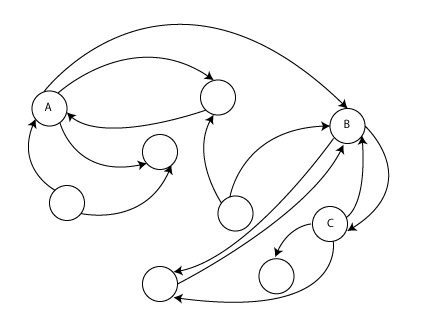
\includegraphics[scale=0.5]{images/ex3.png}
\end{figure} 
\end{homeworkProblem}
%----------------------------------------------------------------------------------------
%	Problem 4
%----------------------------------------------------------------------------------------
\begin{homeworkProblem}[Exercise 3.9]% Custom section title
\vspace*{10pt} % Question 
Write a simple single-threaded web crawler. Starting from a single input URL
(perhaps a professor's web page), the crawler should download a page and then
wait at least five seconds before downloading the next page. Your program should
find other pages to crawl by parsing link tags found in previously crawled documents.
%--------------
%  P4 Approach
%--------------
\subsection{Approach}
Python script \textit{crawler.py}, shown on Listing \ref{listing:crawler}, was developed to complete this exercise. This problem can be divided into the following sub-problems:
\begin{enumerate}
\item Extract Links: Given the representation of a given resource, all the links within that object are extracted for further analysis.
\item Validate Links: \textit{crawler.py} trusts the information provided by the server. ONLY objects with a Content-type value of ``text/html'' and a 200 response code are accepted. Redirects (RC 301 or 302) are followed to the pointed location.
\item Track Crawled Links: This sub-problem is critical in the implementation to avoid an indefinite loop when two or more links point to each other. This was accomplished by keeping a hash list with URLs already crawled.
\end{enumerate}
%--------------
%  P4 Extract Links
%--------------
\subsubsection{Extract Links}
\textit{Crawler.py} uses \textbf{Python} library \textit{BeautifulSoup} to extract all the links from returned object. There are other details that  \textit{crawler.py} takes care off to optimize the extraction before going through the validation step, such as ensuring the URL ends with a backslash and that its schema is accurate. Lines 46-63 take care of link extraction in \textit{crawler.py}.
%--------------
%  P4 Validate Links
%--------------
\subsubsection{Validate Links}
The validation is done by inspecting the header returned by the Webserver. The first validation (line 70) ensures the representation is not for an image, pdf, text file, etc. It ONLY accepts HTML content. If the resource is available, the server will send a response code 200. Only then, that link is crawled (lines 71-72). There are times where the resources are moved to a different location pointed by the URL. If the server has this information, a status code 301 or 302 is sent back to the client requesting that page. \textit{Crawler.py} validates this response 71-87. The iteration is performed until a valid location is reached (response 200) or a different response code is given by the server.

%--------------
%  P4 Track Crawled Links
%--------------
\subsubsection{Track Crawled Links}
It is very common for webpages in a lower hierarchy to point to the home page. It is also possible that pages in the same hierarchy point to each other.  If one does not keep track of which pages have been crawled, not only will the process get duplicated, but it also could get into an indefinite loop, as previously stated.  \textit{Crawler.py} first encodes the URL (line 25), and finds out if this hash is in the hash table (line 26). The crawling is recursive, and the condition to end the recursion is when the webpage has already been crawled.
%--------------
%  List Crawler.py
%--------------
\lstinputlisting[language=Python,
                 style=mybox, 
                 captionpos=t,
                 caption={crawler.py},
				 linerange={21-94},
				 firstnumber=21,                  
                 label=listing:crawler,
                 ]
{crawler.py}
\subsection{Solution}
Our single thread \textit{crawler} started on URL $<$\url{http://cs.odu.edu/~mln/}$>$. It spent quite an amount of time looping through the ODU domain. Eventually, it entered an outside domain. The process had to be interrupted since it entered the World Wide Web, and even though, the same link does not get crawled twice, there were many requests to crawl the same page.
\end{homeworkProblem}
%----------------------------------------------------------------------------------------
%	Problem 5
%----------------------------------------------------------------------------------------
\begin{homeworkProblem}[Exercise 3.14]% Custom section title
\vspace*{10pt} % Question 
Write a program to generate simhash fingerprints for documents. You can
use any reasonable hash function for the words. Use the program to detect duplicates on your home computer. Report on the accuracy of the detection. How
does the detection accuracy vary with fingerprint size?
%------------------
%  Approach
%------------------
\subsection{Approach}
Python script \textit{simhash.py}, shown on Listing \ref{listing:simhash}, was developed to complete this exercise. We used three files: data1.txt, data2.txt and data3.txt (uploaded in Github). They are read and pass as a reference to \textit{simhash.py}. The first two data files were modified slightly to simulate a plagiarism, while the third file is completely different. We can divide this problem into the following sub-problems:
\begin{enumerate}
\item Remove Stop Words
\item Hash Document Words
\item Apply Simhash Algorithm according with \cite{CroftMetzlerStrohman}
\end{enumerate}
\subsubsection{Remove Stop Words}
Using \textbf{Python} library \textit{stop\_words} gives us the ability to remove all the stops words from our file in one line (21).

\subsubsection{Hash Document Words}
\textit{simhash.py} applies MD5 hash to all the words from the file (line 34). The hash is converted to a binary form (line 35). The preceding zeros in Python are removed, and replaced with a b. That is the reason for taking only the element beyond position 2 in the array (line 35).

\subsubsection{Apply Simhash Algorithm}
The \textit{simhash} algorithm sums the frequency of the words with a value 1 in the hash, and deducts its frequency with a value zero (lines 33-43).
\lstinputlisting[language=Python,
                 style=mybox, 
                 captionpos=t,
                 caption={simhash.py},
				 linerange={19-53},
				 firstnumber=19,                  
                 label=listing:simhash,
                 ]
{simhash.py}
\subsection{Solution}
Below, it is the result of running \textit{simhash}\\

\scriptsize
Starting Time: Wed,  Sep 21, 2016 at 22:11:53\\

10010101011111010100101111100001011011010110100010011101100001110000111100100001101101001011011010100101011100111101010111110101\\
10010101011011010100101111100001011011010110100010011101100001110000111100100001101101001011011010101111011101110111010111110101\\
10000100111001110111111101010001110111010011110010101000000010100100010001100100101011101011111111100010100110110110001011010000\\

End Time:  Wed,  Sep 21, 2016 at 22:11:53\\
Execution Time: 0.06 seconds\\

\normalsize
We can notice that the first two hashes are very similar, almost identical. While the third hash is very distinct from the rest.
\end{homeworkProblem}
%----------------------------------------------------------------------------------------
%	Bibliography
%----------------------------------------------------------------------------------------
\newpage
\bibliography{bibliography}
\bibliographystyle{siam}
%\begin{thebibliography}{9}
%\bibitem{Lutz} 
%Lutz, Mark (2013). List and Dictionaries. \textit{Learning Python} (5th ed.). (pp. %262-263). Sebastopol, CA: O'Reilly Media.
%
%\bibitem{ci}
%Segarn, Toby. Programming Collective Intelligence. \textit{Building Smart Web 2.0 Application}. (pp 29-53). Sebastopol, CA: O'Reilly Media.

%\bibitem{sitemaps}
%Sitemaps Schema. (n.d.) Retrieved September 21, 2016, from \url{http://www.sitemaps.org/schemas/sitemap/0.9}

%\end{thebibliography}
\end{document}

